

\section{Predicción }

  	
  En esta sección se presenta formalmente framework que se utilizará durante este trabajo. %@todo: colocar referencia web
  PredictionIO es un servidor de Machine Learning Open Source para Cientistas de Datos y Desarrolladores que permite crear motores de predicción para ambientes de producción, con un bajo tiempo de entrenamiento y despliegue en ambientes productivos. Principalmente esta construido en Apache Spark, HBase y Spray.

  Como ya se ha señalado este ambiente de trabajo se encuentra en un maduración completa que permite tanto disponer  servidores con motores predictivos, como también toda una infraestructura distribuida para hacer que complejos algoritmos sean utilizados para solucionar problemas reales.



% PIO, tiene practicamente todo armadao, ello no hicieron nada nuevo ... solo juntaron  todo...
% MLIB,SPARK, HBASE,SPRAY hadoop etc...
% por lo que he leido es bien similar a java y mas funcional como lenguaje.


% He estado investigando y revisando documentación, Yelp, Skype, Hubot de github y otras implementaciones tienen usando prediction.io




% La otra opción es meterle a este "DASE" un algoritmo  que mezcle una representación de cadenas de markov mezclado con LZ78. no se en que punto mezclarlo en el diccionario, o la verdad es como hacer el compresor sea "mas inteligente", encontré un papaer que te adjunto en el cual usan lz78 y lzw, esta interesante ya que le hacen un acercamiento mas al tema de de ser un predictor online.


% Ahora entiendo que la cadenas de markov son y se han ocupado para las predicciones, pero no veo la necesidad de ocuparlas mayormente. Adin me inisiste en que le de una vuelta.... pero mi sensación  es que tengo separada las ideas en dos extremos. 
% Ya revise Suffix Tree para predicciones LZ77 y LZW, también PPM y HMM.

% Ahora entiendo lo que me dijsite de espantanamiento, como que en la literatura no hay mezcla directa de estas dos areas, he leido "invitaciones a colaborar", pero como que funcionan a la par.

% El otro tema que estoy un poco asustado son el dataset de prisa, ya que no estoy seguro que el formato me sirva 100% con predicction.IO, al fin y al cabo es como medio loco "entrenar a un compresor para que sea inteligente o no" ????




\subsection{Arquitectura DASE}


Un motor de predicción es un tipo de proceso en Machine Learning. Siguiendo una arquitectura de tipo {DASE}, contendríamos los siguientes componentes.



\begin{itemize}

  \item \textbf{ $[D]$ Data Source y Data Preparator }\\
  Los Data Source leen la data desde la entrada original y la transforma en un formato deseado para hacer análisis de estos. En cambio \emph{Data Preparator} pre-procesa la información y la reenvía a los algoritmos para   hacer el modelo de entrenamiento.


    \item \textbf{ $[A]$ Algoritmo}\\
  Los componentes de algoritmos incluyen algoritmos de Machine Learning, estos por los componentes que son de predicitionIO pueden ser provistos por Apache Spark ó se pueden incluir algoritmos propios como también de terceros.
  Adicionalmente a los algoritmos podemos asignarle parámetros, para determinar como debiese ser construido el modelo predictivo.



    \item \textbf{ $[S]$ Servicio}\\
  The Serving component takes prediction queries and returns prediction results. If the engine has multiple algorithms, Serving will combine the results into one. Additionally, business-specific logic can be added in Serving to further customize the final returned results.

    \item \textbf{ $[E]$ Evaluación de Métricas}\\
  Las métricas de evaluación cuantifican la precisión de la predicción con una puntuación numérica. Puede ser utilizado para la comparación de algoritmos o ajustes de los parámetros del algoritmo.


\end{itemize}




\tikzstyle{decision} = [diamond, draw,text width=4.5em, text badly centered, node distance=2.5cm, inner sep=0pt]
\tikzstyle{block} = [rectangle, draw,text width=5em, text centered, rounded corners, minimum height=4em]
\tikzstyle{line} = [draw, very thick, color=black!50, -latex']
\tikzstyle{cloud} = [draw, ellipse, node distance=2.5cm,
    minimum height=2em]

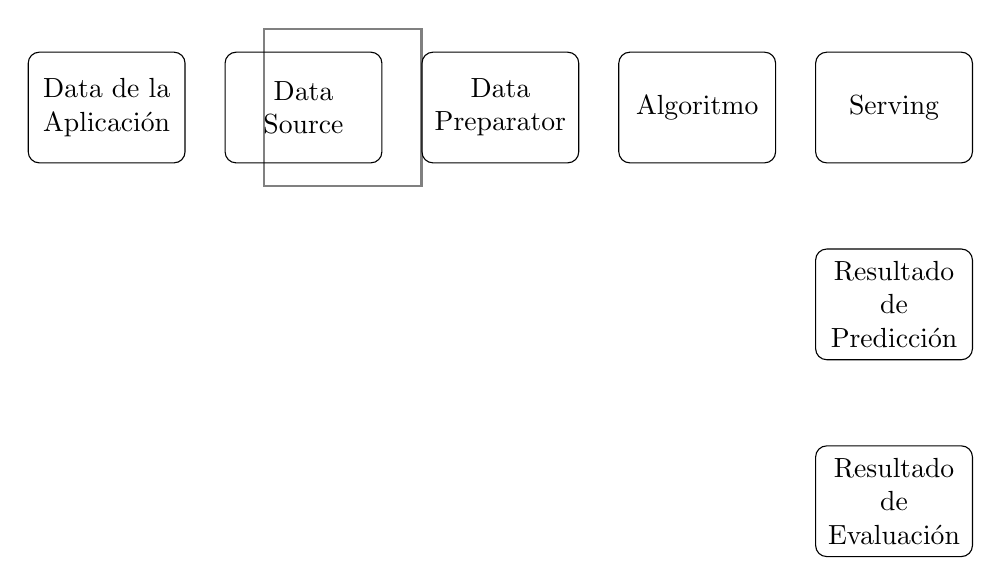
\begin{tikzpicture}[scale=1, node distance = 2.5cm, auto]
    % Place nodes

    \node [block] (init) {Data de la Aplicación};
    
\draw [color=gray,thick](2,-1) rectangle (4,1);    
    \node [block, right of=init] (datasource) {Data Source};
    \node [block, right of=datasource] (datapreparator) {Data Preparator};


    \node [block,right of=datapreparator] (alg1) {Algoritmo };

    \node [block,right of=alg1] (serving) {Serving};

    \node [block,below of=serving] (resultpredict) {Resultado de  Predicción};
    \node [block,below of=resultpredict] (resulteval) {Resultado  de Evaluación};


    % \node [cloud, left of=init] (expert) {expert};
    % \node [cloud, right of=init] (system) {system};

    % \node [block, below of=init] (identify) {identify candidate models};
    % \node [block, below of=identify] (evaluate) {evaluate candidate models};
    % \node [block, left of=evaluate, node distance=2.5cm] (update) {update model};
    % \node [decision, below of=evaluate] (decide) {is best candidate better?};
    % \node [block, below of=decide, node distance=2.5cm] (stop) {stop};
    

    % Draw edges
    % \path [line] (init) -- (identify);
    % \path [line] (identify) -- (evaluate);
    % \path [line] (evaluate) -- (decide);
    % \path [line] (decide) -| node [near start, color=black] {yes} (update);
    % \path [line] (update) |- (identify);
    % \path [line] (decide) -- node [, color=black] {no}(stop);
    % \path [line,dashed] (expert) -- (init);
    % \path [line,dashed] (system) -- (init);
    % \path [line,dashed] (system) |- (evaluate);


\end{tikzpicture}




PredictionIO ayuda a tener  componentes modulares de fácil uso, que hemos descrito  para que se puedan construir modelos de predicción de manera mas sencilla, también poder integrarlos con gran facilidad a cualquier sistema o plataforma, por ejemplo, es posible elegir cual de todos los componentes se podrá desplegar al momento de crear un \emph{Engine} (Motor de Predicción.)




\textbf{Despliegue de Engine}

  Un Engine pone todos los componentes \emph{text}{DASE} en un estado especifico de despliegue

  \begin{enumerate}
    \item Data Source
    \item Data Preparator
    \item Un o más Algoritmos
    \item Un Servicio
  \end{enumerate}

  Si se especifica más de un algoritmo, cada uno de los resultados de los modelos de predicción se entregará para ser consumido por cualquier cliente.
  Cada \emph{Engine} procesa los datos y construye modelos predictivos de forma independiente. Por lo tanto, todos los Engine sirven a su propio conjunto de resultados de predicción. Por ejemplo, puede desplegar dos Engine para su aplicación móvil: uno para recomendar noticias para los usuarios y otro para sugerir nuevos amigos a los usuarios.



\textbf{Evaluación del Engine }

  Para evaluar el Accurracy de un Engine, solo se debe especificar la métrica cuando se corre el motor de evaluación, en los capítulos experimentales usted podrá ver como se generan estás métricas y como se usa este motor de predicción.











\subsection{Modelamiento de Eventos}

%https://docs.prediction.io/datacollection/eventmodel/


\textbf{Modelamiento de Eventos}

  El modelamiento de eventos, es simplemente el hecho de poder llevar un feature\footnote{Característica de un cierto dataset para entrenar.}   que es del mundo del ML, es en fin una representación de como se debe tener la data de manera RDD para poder acceder a ella posteriormente. 

  Un evento lo definiremos como entidad que nos permite dar una representación temporalizada de información la cual será procesada por un motor de predicción. Analizaremos los eventos que un usuarios realiza para poder acceder a una web. Adicionalmente cuando cada usuario ingresa a una web automáticamente este genera un sesión, la cual es desde que que llega hasta que abandona la web.

  Como ya se ha mencionado en sección anteriores esta información esta totalmente depurada y entregada por los access log, los cuales a efectos de temporalidad nos interesa conocer la secuencialidad discreta de estos accesos.
  


%Poner algo mas matematico.
% EVENT API 
% https://docs.prediction.io/datacollection/eventapi/

  El modelamiento que se realizará contempla que el usuario :


    \begin{itemize}
      \item Tipo de Evento: Visitar
      \item Entidad que ejecuta el evento: Usuario
      \item Propiedades:
          \begin{enumerate}
            \item Pagina actual
            \item Pagina siguiente
            \item Cierre de Sesión
          \end{enumerate}
    \end{itemize}



    El interés de tener un modelo totalmente atómico es poder contemplar la información que nos entrega, destacando sus variables y propiedades como restricciones.



\subsection{Ventajas }


  Es posible mezclar y aplicar distintas característica si el modelo no puede ser ser persistido por PredictionIO automáticamente. Se requiere un objeto acompañante heredada de una clase que permite lograr la persistencia en memoria (IPersistentModelLoader ), esto permite PredictionIO  cargar el modelo persistentemente y automáticamente durante la implementación.

  % Tenga en cuenta que los modelos generados por PAlgorithm no pueden ser persistieron automáticamente por naturaleza y deben implementar estas características, si se desea modelo de persistencia.


  Comprendiendo el concepto de RDD, esta es la abstracción básica de Spark, aún más esto es una de las grandes cualidades de PredictionIO, ya que no solamente podemos disponer de un máquina para hacer estudios o implementar algoritmos, este servidor de Machine Learning permite gracias a sus componentes poder hacer un cluster para lograr entregar mayor eficiencia acorde a los datos o algoritmo a implementar.  Esta propiedades

  Ya hemos mencionado que un \emph{Resilient Distributed Dataset} (RDD) es un representación inmutable, una colección particionada de elementos que pueden ser operadas en paralelo. Internamente cada RDD tiene cinco principales propiedades:


  \begin{enumerate}
    \item Una lista de particiones.
    \item Una función para procesar cada split de datos.
    \item Una lista de dependencias en otros RDD's. 
    \item Opcionalmente una partición de un RDD puede ser representada como $\{llave,valor\}$ 

    \item Opcionalmente, una lista de los lugares preferidos para calcular cada una dividida en (por ejemplo, lugares de bloque para un archivo HDFS), para procesamiento en Clustering.

  \end{enumerate}




% https://docs.prediction.io/templates/recommendation/customize-serving/
















